\documentclass[12pt,letterpaper]{article}
\usepackage[utf8]{inputenc}
\usepackage{amsmath}
\usepackage{amsfonts}
\usepackage{amssymb}
\usepackage{fancyhdr}
\usepackage{graphicx}
\usepackage[left=0.79in, right=0.79in, top=0.79in, bottom=0.79in]{geometry}
\author{Chathan Driehuys}

\graphicspath{{./images/}}

\pagestyle{fancy}
\lhead{COMP 535}
\chead{Return To Lib-C}
\rhead{Chathan Driehuys}

\begin{document}
	\section*{Task 1}
		The first step in getting access to a root shell was to overflow the buffer in \texttt{retlib.c} to overwrite the return address. In order to gain shell access, the \texttt{system} function needed to be invoked, so we had to overwrite the return address from \texttt{bof} to be the location of the \texttt{system} function.
		
		To find the location of the \texttt{system} function we simply printed its address using the debugger. Finding the return address' offset from the start of the buffer being overflowed involved a little more trial and error, but was fairly straight forward with \texttt{gdb}.
		
		After exploiting the stack to make call \texttt{system}, we used the debugger once more to find the location of the return address for that frame. We were then able to insert the address of the \texttt{exit} function.
		
		The final problem was locating the \texttt{/bin/sh} value stored in an environment variable. Utilizing the debugger, we used the following command to get an address for the desired string:
		
		\begin{verbatim}
			(gdb) p /x getenv("MYSHELL")
			<address of $MYSHELL>
		\end{verbatim}
		
		After adjusting offsets so that we only received the value of the environment variable, we then had to find where to insert the value. Since the first 12 bytes of the buffer do not overflow, we knew it had to be placed outside that range. The offsets of 24 and 28 bytes were already taken by the \texttt{system} and \texttt{exit} addresses, so it was simply a matter of trying the remaining offsets: 16, 20, 32, and 36 bytes. Trial and error led to the end result of a 32 byte offset for the \texttt{/bin/sh} parameter passed to \texttt{system}.
		
		\begin{figure}[h]
			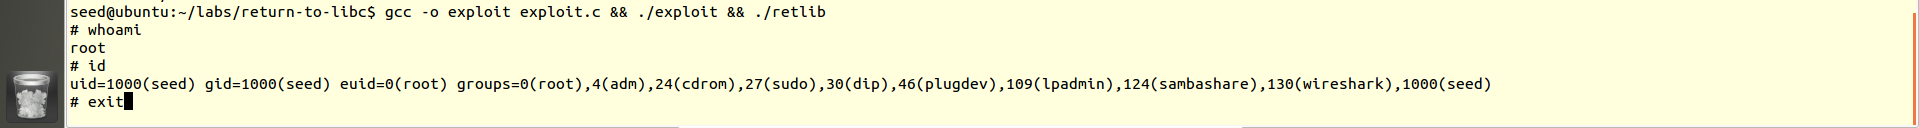
\includegraphics[width=\linewidth]{task-1}
			\caption{Obtaining a root shell using a return-to-libc attack.}
		\end{figure}
		
		Changing the name of the binary from \texttt{retlib} to \texttt{newretlib} caused our attack to fail.
		
		\begin{verbatim}
			seed@ubuntu:~/labs/return-to-libc$ ./newretlib 
			sh: 1: h: not found
		\end{verbatim}
		
		The error message indicates that the increased length of the filename throws off the address of the environment variable used to obtain the \texttt{/bin/sh} value passed to the \texttt{system} function.
	
	\section*{Task 2}
		When enabling address space randomization, we no longer know the correct offsets to insert our desired return addresses at so our exploit no longer works. Because this style of attack depends on overwriting multiple addresses in specific locations, this protection is particularly effective.
		
		\begin{verbatim}
			seed@ubuntu:~/labs/return-to-libc$ ./retlib
			Segmentation fault (core dumped)
		\end{verbatim}
		
	\section*{Task 3}
		Enabling the ``stack guard'' has no effect on this exploit. Because this attack does not execute any instructions inserted onto the stack, it works regardless of whether or not the stack is executable. This is the benefit of the ``return-to-libc'' style of attacks which execute existing code by manipulating addresses rather than instructions.
\end{document}